\chapter{Functional Advantages of Rich Spatiotemporal Searching Dynamics}\label{chap:functional_advantages}
The true advantage of having a biologically realistic functional model of eye movements is that we can examine the informational advantages of each dynamical component studied. A major motivation for this study is that previous work have shown that eye movements are well predicted by ``greedy'' informational-maximisation strategies, especially in \textcite{Renninger2005-ee} along with later sophisticated developments from \textcite{zhu_autocorrelated_2024, butko_infomax_2010}. Thus, we aim here to show that the macroscopic dynamical signatures described in \cref{chap:a_unifying_model} and their validated in human gaze dynamics in \cref{chap:empirical_validations} play functional roles from an abstract probabilistic sampling perspective. Motivated by the construction of this model as accounting for gaze dynamics, we consider the same search task as defined in \cref{sec:model_setup}. However, each of the metrics and methods may be used in high dimensional probabilistic sampling tasks, or during search exploration of a dynamical landscape. Each dynamical component described has analogy to a feature of abstract sampling algorithms: kernel-driven adaptation will improve ergodicity and can be compared to metadynamics \cite{tiwary_time-independent_2015,bussi_using_2020,barducci_well-tempered_2008}, local harmonic oscillations can be compared to the fast mixing and negative autocorrelation in sampling found in Hamiltonian Monte Carlo \cite{betancourt_conceptual_2018, Ottobre2016-xp} and second-order Langevin sampling methods \cite{liu2025secondorderensemblelangevin, Ottobre2016-xp}, and finally Lévy superdiffusion has gathered a growing body of literature as a robust sampling strategy which does not require fine-tuning to explore unknown heavy-tailed or multimodal distributions \cite{simsekli_fractional_nodate, ijcai2018p419, oechsler_levy_2024, behme_levy_2026}.

The first section of this chapter (\cref{sec:information-theoretic_metrics}) presents informational-theoretic methods which have been constructed to analyse efficiency during abstract search tasks. Key to this method is the quantification of information of a belief distribution as the distribution entropy $S_{\pi} = -\int_{\textbf{x}} d\textbf{x} \ln \pi(\textbf{x})$, and tracking its development through a search task. The second section (\cref{sec:functional_roles_of_dynamical_patterns}) takes these metrics and compares the informational advantages from dynamics driven in parameter space $\alpha/\beta/\gamma/\tau$. The final section (\cref{sec:further_extensions_of_studied_dynamic}) examines further extensions of these dynamics beyond the case of 2-dimensional visual search to high-dimensional or dynamical target landscapes, where control and exploration are hypothesised be more responsive and robust to shifts in a loss function.

%%% 4.1 Information-theoretic metrics
\section{Information-theoretic metrics}\label{sec:information-theoretic_metrics}
When considering the efficiency advantages of strategic sampling in a visual search task, the central quantity under study is the information gain, $IG(t)$. To quantify informational search efficiency across a full abstract search landscape, we take inspiration from Bayesian inference and sampling methods. In particular, the adaptive dynamics of our sampling model closely resemble well-tempered metadynamics in Markov chain Monte Carlo (MCMC) sampling \cite{tiwary_time-independent_2015}. Simultaneously, similar techniques have been applied to model visual search in discrete time by tracking the information gathered strictly at a target goal position \cite{bujia_modeling_2022}. In \cref{sec:dynamical-information_adaptation} we have expanded and unified these approaches by analysing a continuous-time behavioural dynamical-information kernel. By tracking and integrating real-time kernel deposition at every location in the informative landscape, we model global information acquisition across an evolving landscape of belief. 

\subsubsection*{Quantifying kernel-driven dynamical information}
To encode this potential function adaptation, we take inspiration from Bayesian inference and sampling methods. In particular, the dynamics are very similar to the foundational technique of well-tempered metadynamics in MCMC sampling \cite{tiwary_time-independent_2015}. The application of such a technique to modelling studies of a visual search has been described in discrete time by \textcite{bujia_modeling_2022}, where the equivalent target distribution is the likelihood distribution for some search goal. In this work, the information is only tracked at the goal position, by tracking the likelihood value at this point. However, we expand on this work by analysing the information kernel in our continuous-time model, and tracking the posterior target distribution after kernel deposition at every location in the visual scene, thus tracking global information acquisition. 

We quantify this information across the entire target landscape gained through this adaptive kernel. In particular, given the theoretical paradigm of a search through a probabilistic landscape for high probability modes, information extracted is proportional to the change in entropy of the target distribution. Since we study an update to an effective belief distribution (where target likelihood is the likelihood of locating a goal), we directly use the language and tools of Bayesian inference. Examining the cross-entropy of the landscape at some time $t$ (the posterior distribution $\pi_t(\textbf{x})$) to the original pre-search landscape (the prior distribution $\pi_0(\textbf{x})$) is the natural first step in comparing information gathering through time.

Considering the initial pre-search belief distribution, $\pi_0(\textbf{x})$, we examine the information gained in kernel updates to $\pi_t(\textbf{x})$. $\pi_0(\textbf{x})$ can be defined through $V_0(\textbf{x})$, which functions as the saliency-potential landscape, through Boltzmann-Gibbs statistics
\begin{equation}
    \pi_0(\textbf{x}) = \frac{\exp\{-V_0(\textbf{x})\}}{\int_{\textbf{x}'} \exp\{-V_0(\textbf{x}')\} \, d\textbf{x}'}
\end{equation}
As the visual search progresses, the initial effective potential $V_0(\textbf{x})$ updates in continuous time to encode learned information. This adaptation takes the form of an accumulated kernel over time $t$:
\begin{equation}
    V_t(\textbf{x}) = V_0(\textbf{x}) + \int_0^t k(\textbf{x}_{t'}) \, \frac{dt'}{\tau}
\end{equation}
This adapted potential defines the posterior belief distribution, representing the updated target likelihood landscape at time $t$
\begin{equation}
    \pi_t(\textbf{x}) = \frac{\exp\{-V_t(\textbf{x})\}}{\int_{\textbf{x}'} \exp\{-V_t(\textbf{x}')\} \, d\textbf{x}'}
\end{equation}
Because these dynamics study updates to an belief distribution—where likelihood reflects the probability of locating a goal—we directly utilise the analytical framework of Bayesian inference to measure efficiency. Given the search through a probabilistic landscape for high-probability modes, the information extracted is proportional to the change in the distribution's entropy. A natural first step in evaluating information gathering over time is to compute the cross-entropy between the posterior distribution $\pi_t(\textbf{x})$ and the prior distribution $\pi_0(\textbf{x})$:
\begin{equation}
    H(\pi_t, \pi_0) = -\int \pi_t(\textbf{x}) \log \pi_0(\textbf{x}) \, d\textbf{x}
\end{equation}
However, it has been found that cross-entropy alone is of limited utility, as it conflates the internal concentration of belief within the posterior (represented by its self-entropy, $H(\pi_t)$) with the net information gained relative to the prior. To decouple these two contributions, we subtract the posterior entropy term to obtain the Kullback-Leibler (KL) divergence, $D_{\text{KL}}(\pi_t \parallel \pi_0)$. This yields the formal definition of information gain up to time $t$:
\begin{align}
    IG(t) &= H(\pi_t, \pi_0) - H(\pi_t) \nonumber \\
          &= -\int \pi_t(\textbf{x}) \log \pi_0(\textbf{x}) \, d\textbf{x} + \int \pi_t(\textbf{x}) \log \pi_t(\textbf{x}) \, d\textbf{x} \nonumber \\
          &= \int \pi_t(\textbf{x}) \log \left( \frac{\pi_t(\textbf{x})}{\pi_0(\textbf{x})} \right) d\textbf{x} \nonumber \\
          &\equiv D_{\text{KL}}(\pi_t \parallel \pi_0) \label{eq:information_gain}
\end{align}
Two fundamental properties of the KL divergence are that it is non-negative and asymmetric. In the context of an abstract sampling model, the non-negativity represents the fact that any spatial update from $\pi_0$ represents accumulated evidence, though not necessarily optimal search efficiency. A weak kernel, slow informative timescale $\tau$, or deposition in low-likelihood areas alters the landscape only marginally and results in slower growth in $IG$. The information content of the search trajectory is therefore entirely captured by $IG$, quantifying the global information acquired as the observer's belief landscape evolves from $\pi_0$ to $\pi_t$.
\subsubsection*{Information velocity}
A direct quantity derived from the definition of information gain is information velocity $IV$. The information velocity is defined directly as the first derivative of $IG$. Comparing the averaged value of the information velocity given the same informative timescale $\tau$ measures how different strategies serve to quantify the quality of information gathered. A strategy targeting high likelihood areas, and driving transitions which are sensitive to the decrease in level of likelihood will have high average $IV_{\text{mean}}$ and $IV_{\text{med}}$ values.
\subsubsection*{First passage time}
Perhaps the clearest metric of search efficiency is the speed of completing a task. In our system, this is calculated directly as the duration of each trial, called first passage time (FPT). We can derive an expected first passage time based on the theta-scale rate of saccades as calculated in \cref{eq:theta_rhythm} under \cref{sec:dynamical-information_adaptation} and the amount of target points in the visual scene compared to the total. Using a number of targets $K$, and a total number of points $N$, the probability of reaching no targets after $n$ saccades is given by the hypergeometric distribution evaluated at zero:
\begin{equation} \label{eq:hypergeo}
    p_n(0) = \frac{\binom{K}{0}\binom{N-K}{n}}{\binom{N}{n}} = \frac{(N-K)!(N-n)!}{(N-K-n)!N!}
\end{equation}
To find the expected number of saccades $\mathbb{E}[n]$, we calculate for which $n$ \cref{eq:hypergeo} gives $p_n(0)<0.5$. The expected first passage time is then $\mathbb{E}[\text{FPT}] = t_{\theta} \mathbb{E}[n]$. For our standard set of parameters and experiment as defined in \cref{chap:model_fitting}, we can see that this gives an expected first passage time
\begin{align}
    \mathbb{E}[\text{FPT}] &= t_{\theta} \times \mathbb{E}_{N=256,K=5}[n] \nonumber \\
    &= 0.1422 \times 94 \nonumber \\
    &= 13.36 \ \text{secs}\label{eq:fpt_expected}
\end{align}
This calculation assumes that each transition is independent and drawn from a stationary distribution with mean $t_{\theta}$ across the search task. These assumptions expect the true dynamics of the system to yield an averaged FPT value that depends on the system parameters. For instance, a superdiffusive walker will have access to the entire scene and may explore nearby fixation points, and then migrate to far-displaced areas of the scene. Another consideration is the strength of the memory-momentum term $\beta$, linked to the gamma-scale fixational tremor of physiological eye tracking data. This activity may allow a more responsive reaction to changes in the saliency landscape as information is received from the scene.
\subsubsection*{Shape parameter}
While the preceding metrics depend explicitly on the search timescale, we can evaluate the fundamental efficiency of a sampling process by making the search timescale dimensionless. By normalising each search trial so that both time and information content range from 0 to 1, we can examine the averaged shape of the monotonic accumulation curve $IG(t)$ independent of absolute time. Statistically, we can calculate an average value for this by considering the area under the information-gain curve and transforming it to examine an effective power law fit of information gain.
\subsubsection*{Gini coefficient}
For a Gini coefficient, we examine the inequality in the information gained over smalled binned time periods, larger than the gamma oscillation
\subsubsection*{Information-entropy gradient}
Here, we attempt to measure the gradient of information to changes in posterior certainty. That is, the efficiency a change in belief has in gaining information


%%% 4.2 Functional roles of dynamical patterns
\section{Functional roles of dynamical patterns}\label{sec:functional_roles_of_dynamical_patterns}

The dynamics that have been studied in this thesis are characterised by three distinct spatiotemporal signatures: gamma-band oscillations, theta-scale rhythmicity, and superdiffusive spatial trajectories. The framework described in \cref{chap:a_unifying_model} from modelling \cref{eq:fns} in a search task aims to unify these signatures as coupled dynamics which provide flexible functional roles in basic computation. In the present section we identify each dynamical pattern with a particular functional role in sampling: local exploitation in gamma oscillations, temporal organisation in theta rhythmicity, and global exploration through $\alpha$-superdiffusion. Using those metrics laid out in \cref{sec:information-theoretic_metrics}, we can precisely identify the functional role and advantages of each dynamical pattern.

\subsection{Gamma oscillations}
At the finest spatiotemporal scales, both FNS dynamics and empirical gaze dynamics are characterised by high-frequency stochastic local sampling. These dynamics are analogous to the gamma oscillations found throughout the brain in almost every computational task. Within our continuous-time dynamical model, local oscillatory behaviour is controlled by the memory-momentum term $p_t$ and the noise driven by $\alpha$-Lévy noise $dL_t^{\alpha}$ within a highly localised potential well.

From an abstract sampling perspective such local oscillations are related to rapid decorrelation of sampled locations, and regular probing of local gradients in the posterior distribution $\pi_t(\textbf{x})$. In the context of visual sampling, this gradient-awareness is associated with contrast and high spatial frequencies, where ocular microtremor has been shown to be beneficial in perception of high spatial frequencies.


The primary functional role of this gamma-scale activity is to continuously probe the local gradient of the posterior belief distribution, $\pi_t(\textbf{x})$. By oscillating rapidly within a confined neighbourhood, the visual system samples local spatial variations in saliency, thereby rendering the search process robust and responsive to the target landscape $V_t(\textbf{x})$. Furthermore, this dynamic momentum allows for a highly responsive reaction to real-time changes in the saliency landscape. As information is rapidly gathered and the kernel incrementally updates the local landscape, local harmonic oscillations enforce sensitivity to gradients of posterior belief distribution $\pi_t$. The important metrics here are the $IV$, $\frac{dIG}{dH}$, and $FPT$.

\begin{figure}[htbp]
    \centering
    \begin{subfigure}[b]{0.33\textwidth}
        \centering
        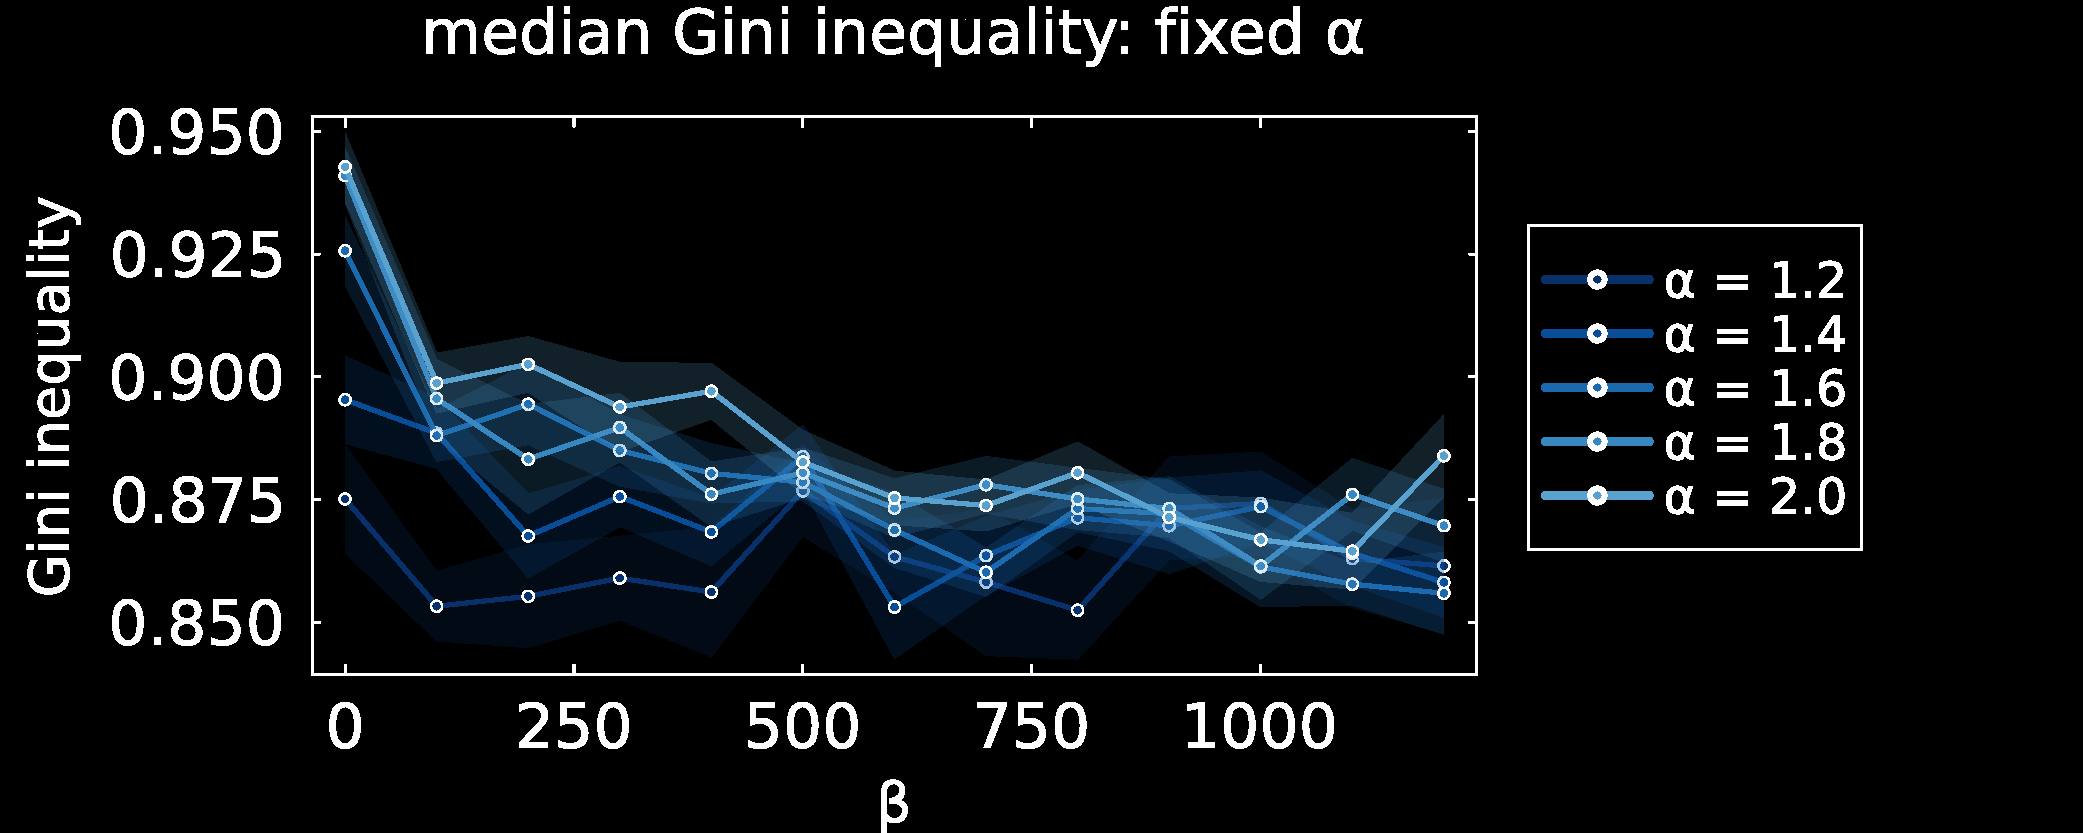
\includegraphics[width=\linewidth]{figures/information_metrics/median_gini_vs_beta.pdf}
        % \caption{\textbf{Rate-corrected rhythmicity index (RCRI) is positively correlated with saccade rate.} Collaborators \textcite{naher_primate_saccades} uncovered this statistically significant result, which implies that shorter inter-saccadic intervals (ISIs) will result in more regular ISIs, which corresponds to stronger kernel dynamics as defined in \cref{sec:adaptive_kernel}.}
        \label{fig:sub1}
    \end{subfigure}
    \vfill
    \begin{subfigure}[b]{0.33\textwidth}
        \centering
        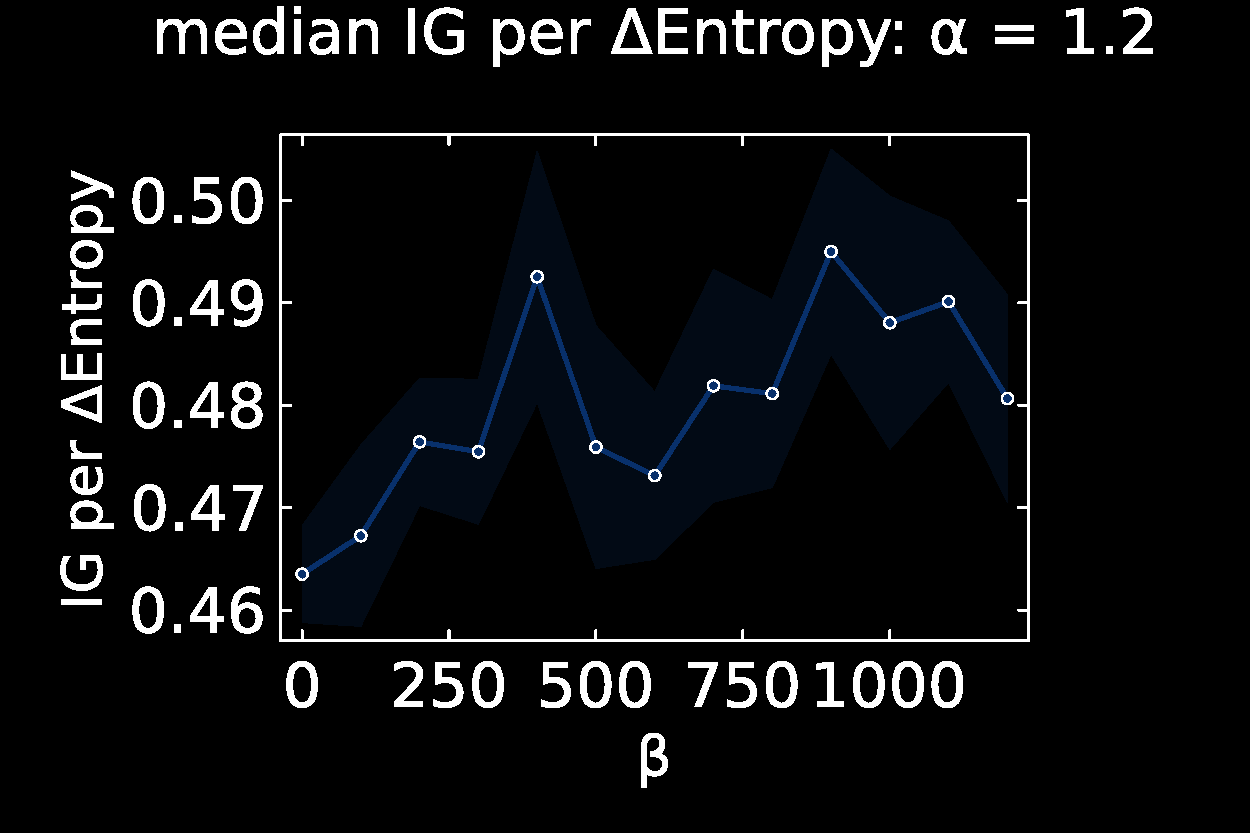
\includegraphics[width=\linewidth]{figures/information_metrics/median_ig_per_dent_alpha1p2_vs_beta.pdf}
        % \caption{\textbf{The probability distribution of inter-saccadic intervals (ISIs) are tightly distributed in a Gamma-10 distribution.} Our collaborators in \textcite{naher_primate_saccades} find that saccades are more locally rhythmic than previously considered. In particular, the ISI distribution is a tight Gamma-10 distribution, but the ISI timeseries is strongly locally rhythmic, as captured by the rate-corrected rhythmicity index (RCRI).}
        \label{fig:sub2}
    \end{subfigure}
    \vfill
    \begin{subfigure}[b]{0.33\textwidth}
        \centering
        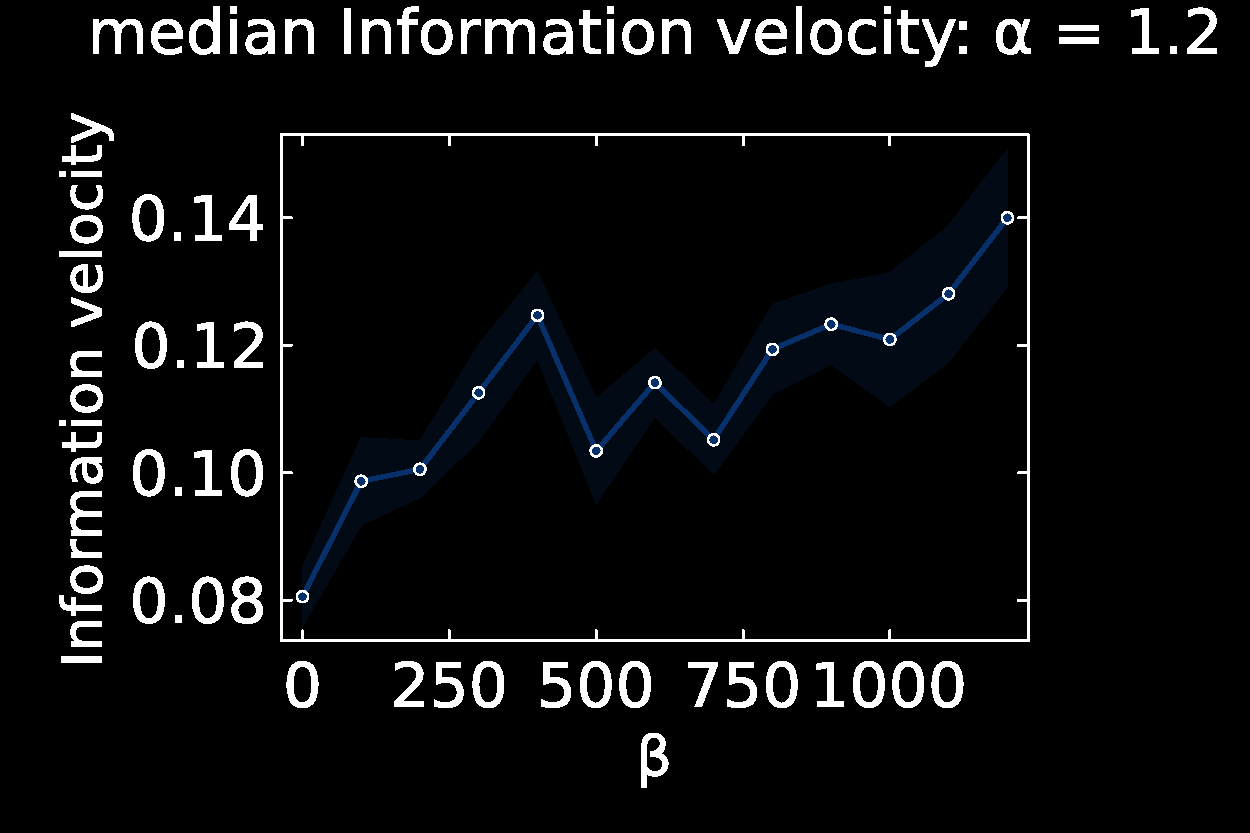
\includegraphics[width=\linewidth]{figures/information_metrics/median_mean_info_velocity_alpha1p2_vs_beta.pdf}
        % \caption{\textbf{The probability distribution of inter-saccadic intervals (ISIs) are tightly distributed in a Gamma-10 distribution.} Our collaborators in \textcite{naher_primate_saccades} find that saccades are more locally rhythmic than previously considered. In particular, the ISI distribution is a tight Gamma-10 distribution, but the ISI timeseries is strongly locally rhythmic, as captured by the rate-corrected rhythmicity index (RCRI).}
        \label{fig:sub2}
    \end{subfigure}
    \vfill
    \begin{subfigure}[b]{0.33\textwidth}
        \centering
        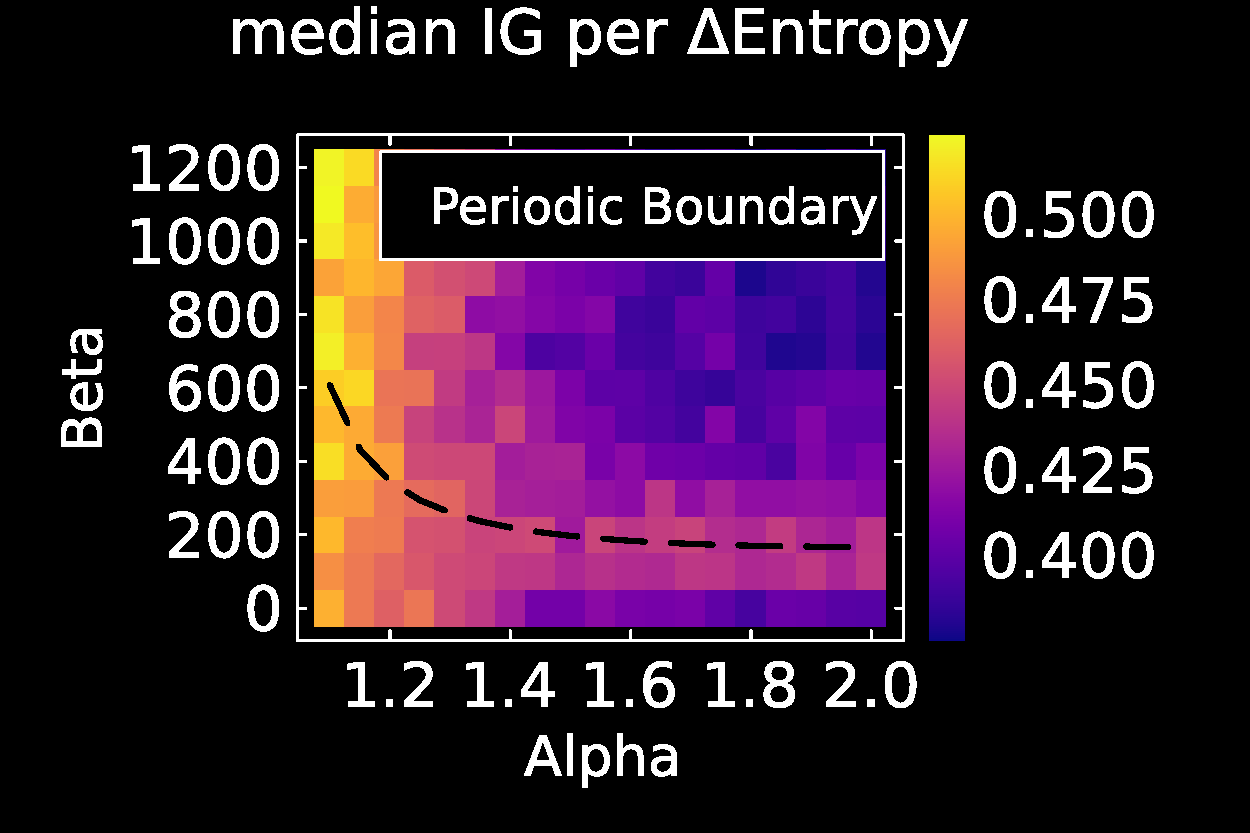
\includegraphics[width=\linewidth]{figures/information_metrics/median_ig_per_dent_heatmap.pdf}
        % \caption{\textbf{The probability distribution of inter-saccadic intervals (ISIs) are tightly distributed in a Gamma-10 distribution.} Our collaborators in \textcite{naher_primate_saccades} find that saccades are more locally rhythmic than previously considered. In particular, the ISI distribution is a tight Gamma-10 distribution, but the ISI timeseries is strongly locally rhythmic, as captured by the rate-corrected rhythmicity index (RCRI).}
        \label{fig:sub2}
    \end{subfigure}
    \vfill
    \begin{subfigure}[b]{0.33\textwidth}
        \centering
        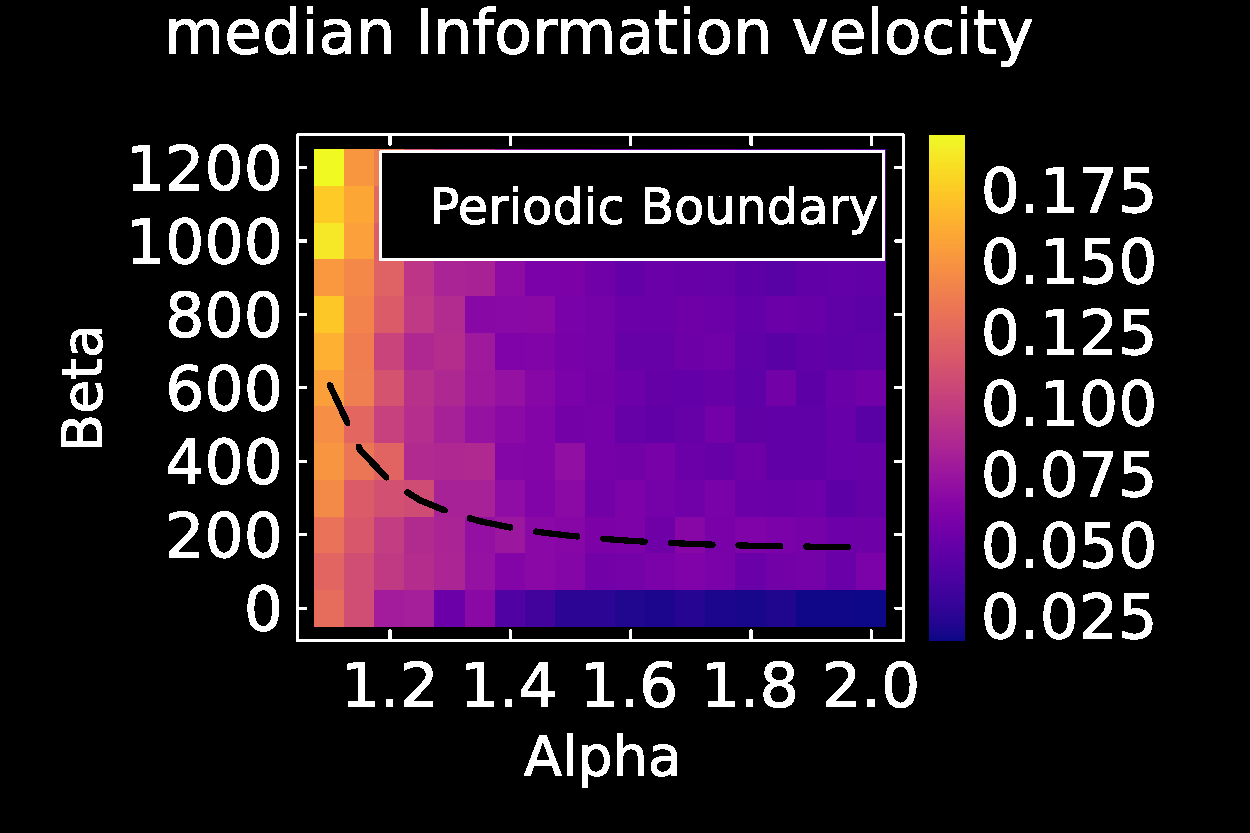
\includegraphics[width=\linewidth]{figures/information_metrics/median_mean_info_velocity_heatmap.pdf}
        % \caption{\textbf{The probability distribution of inter-saccadic intervals (ISIs) are tightly distributed in a Gamma-10 distribution.} Our collaborators in \textcite{naher_primate_saccades} find that saccades are more locally rhythmic than previously considered. In particular, the ISI distribution is a tight Gamma-10 distribution, but the ISI timeseries is strongly locally rhythmic, as captured by the rate-corrected rhythmicity index (RCRI).}
        \label{fig:sub2}
    \end{subfigure}
    \caption{Main figure caption encompassing both subfigures.}
    \label{fig:main}
\end{figure}

\subsection{Theta rhythmicity}
Noise and harmonic neural adaptation dynamics drive local sampling of potential wells, however these periods of local sampling are organised by transitions between sparse areas of high likelihood. Through motion driven by either Lévy- or Brownian noise, transition intervals are exponentially distributed according to a Poisson point process. This is a result of the Lévy-Itô decomposition theorem as presented in \cref{subsec:levy_motion}, where jumps the size of the distance between wells will be Poisson-distributed. However, driving these modal transitions as regular theta-rhythmic events tied to the rate of information acquisition will organise local sampling dynamics to drive higher equality in the amount of information gathered through a cycle of modal exploration.

When testing the effect of theta rhythmic transitions, it is important to examine the dimensionless search effects of varying $\tau$, as $\tau$ directly effects the timescale of information gathering and thus metrics such as $IV$ or $FPT$ will be trivially improved by a decrease in $\tau$.


\subsection{Superdiffusion}
The final dynamical search strategy is superdiffusion, allowing spatially global exploration. Superdiffusive search paths are thought to be optimal when exploring sparse unknown landscapes under the Lévy foraging hypothesis, as described in \cref{subsubsec:anomalous_superdiffusion}. Here, superdiffusion governs the spatial scaling of global exploration, where temporal dynamics of rhythmically organised local sampling of potential wells are explored globally, with superdiffusion allowing long range access to unknown information. 

Scale-free spatial exploration allows the model to rapidly traverse expanses of low-likelihood space. Ultimately, the superdiffusive parameter $\alpha$ is the structural mechanism that prevents the sampler from becoming permanently trapped in a locally depleted belief minimum, ensuring global convergence of the visual inference task. 

\begin{figure}[htbp]
    \centering
    \begin{subfigure}[b]{0.33\textwidth}
        \centering
        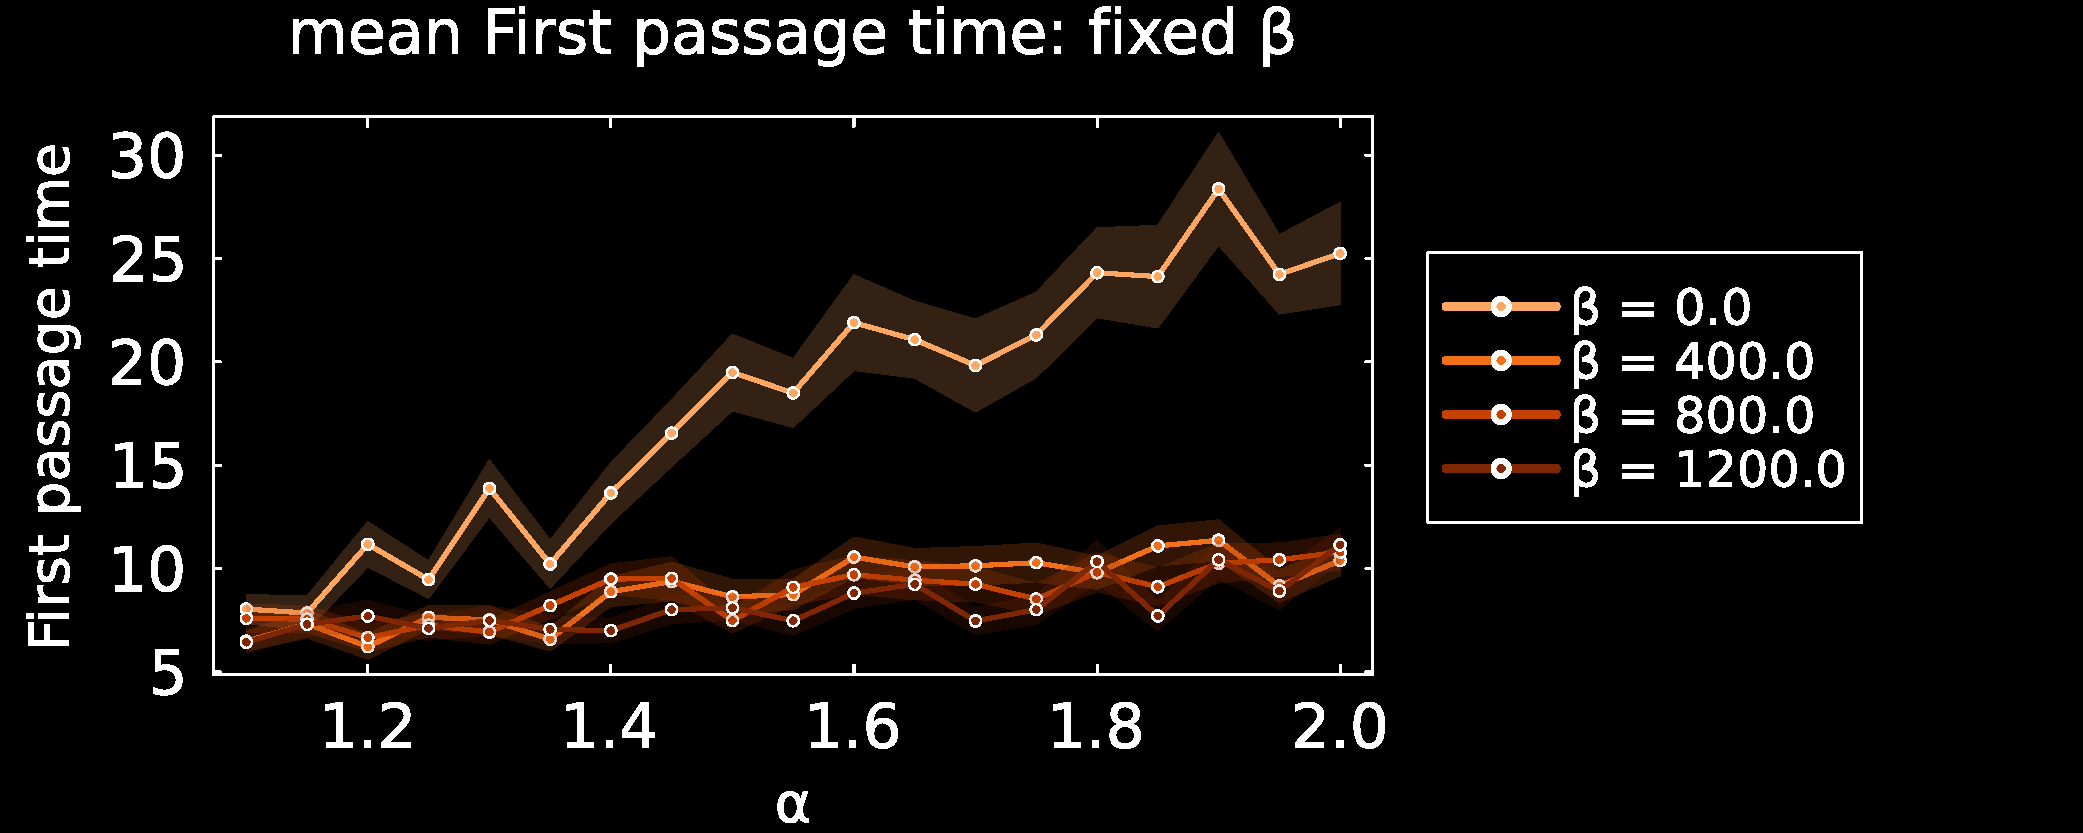
\includegraphics[width=\linewidth]{figures/information_metrics/mean_fpt_vs_alpha.pdf}
        % \caption{\textbf{Rate-corrected rhythmicity index (RCRI) is positively correlated with saccade rate.} Collaborators \textcite{naher_primate_saccades} uncovered this statistically significant result, which implies that shorter inter-saccadic intervals (ISIs) will result in more regular ISIs, which corresponds to stronger kernel dynamics as defined in \cref{sec:adaptive_kernel}.}
        \label{fig:sub1}
    \end{subfigure}
    \vfill
    \begin{subfigure}[b]{0.33\textwidth}
        \centering
        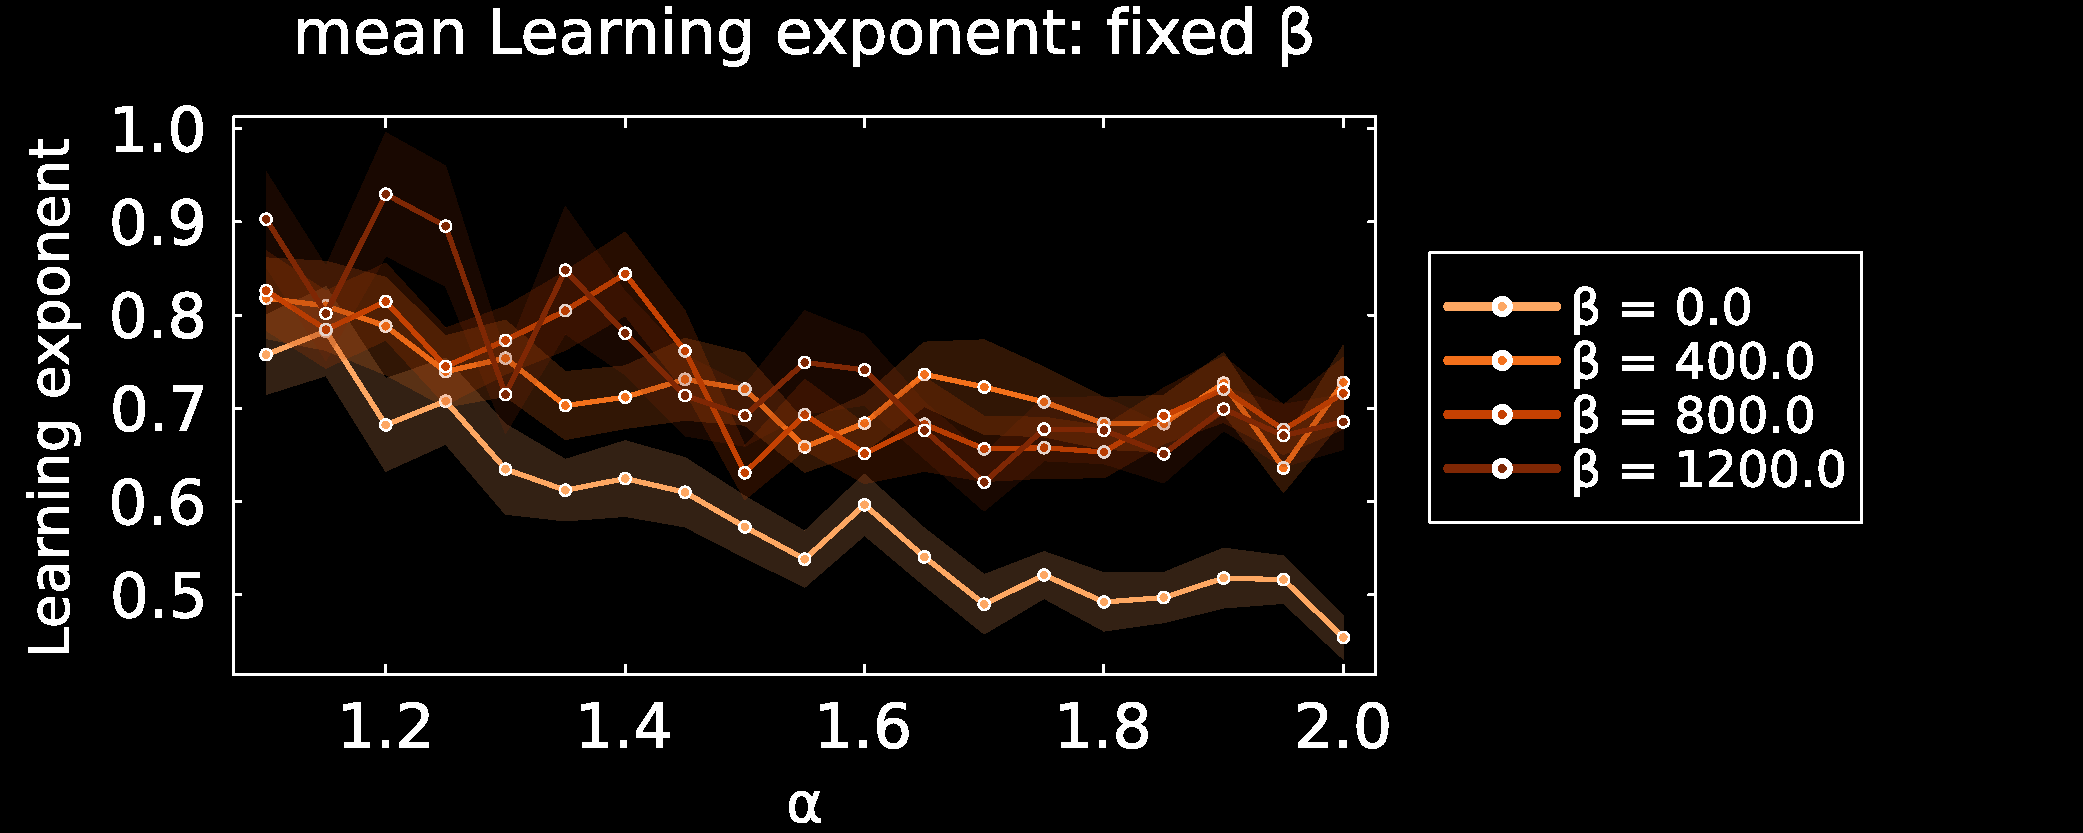
\includegraphics[width=\linewidth]{figures/information_metrics/mean_exponent_shape_vs_alpha.pdf}
        % \caption{\textbf{The probability distribution of inter-saccadic intervals (ISIs) are tightly distributed in a Gamma-10 distribution.} Our collaborators in \textcite{naher_primate_saccades} find that saccades are more locally rhythmic than previously considered. In particular, the ISI distribution is a tight Gamma-10 distribution, but the ISI timeseries is strongly locally rhythmic, as captured by the rate-corrected rhythmicity index (RCRI).}
        \label{fig:sub2}
    \end{subfigure}
    \vfill
    \begin{subfigure}[b]{0.33\textwidth}
        \centering
        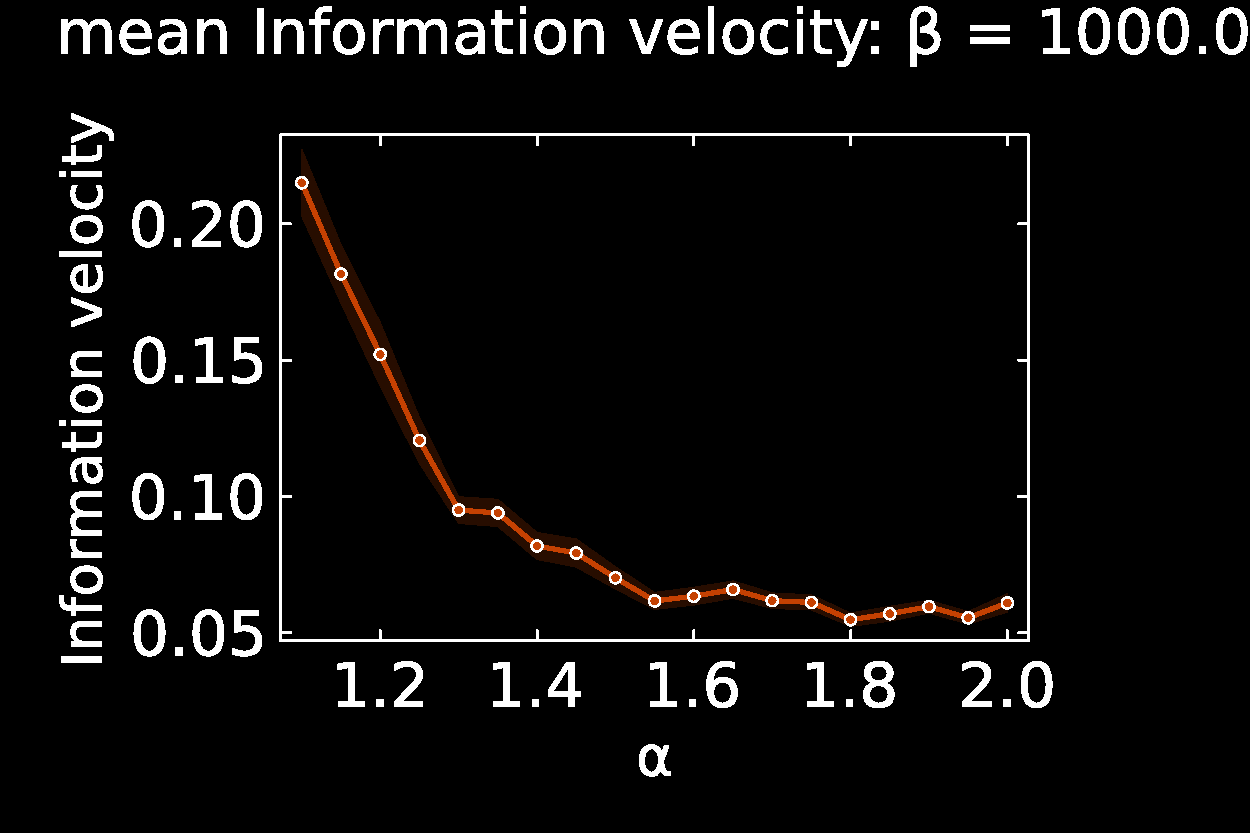
\includegraphics[width=\linewidth]{figures/information_metrics/mean_mean_info_velocity_beta1000_vs_alpha.pdf}
        % \caption{\textbf{The probability distribution of inter-saccadic intervals (ISIs) are tightly distributed in a Gamma-10 distribution.} Our collaborators in \textcite{naher_primate_saccades} find that saccades are more locally rhythmic than previously considered. In particular, the ISI distribution is a tight Gamma-10 distribution, but the ISI timeseries is strongly locally rhythmic, as captured by the rate-corrected rhythmicity index (RCRI).}
        \label{fig:sub2}
    \end{subfigure}
    \vfill
    \begin{subfigure}[b]{0.33\textwidth}
        \centering
        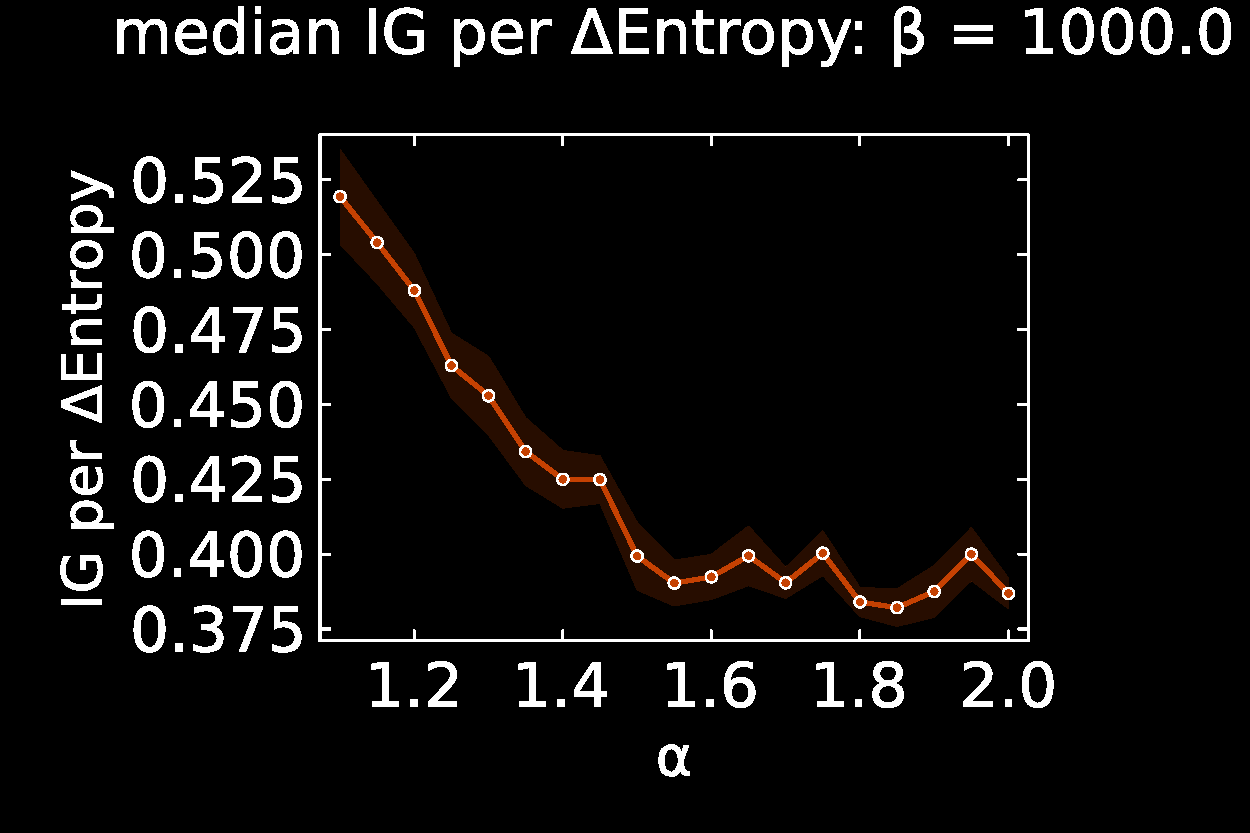
\includegraphics[width=\linewidth]{figures/information_metrics/median_ig_per_dent_beta1000_vs_alpha.pdf}
        % \caption{\textbf{The probability distribution of inter-saccadic intervals (ISIs) are tightly distributed in a Gamma-10 distribution.} Our collaborators in \textcite{naher_primate_saccades} find that saccades are more locally rhythmic than previously considered. In particular, the ISI distribution is a tight Gamma-10 distribution, but the ISI timeseries is strongly locally rhythmic, as captured by the rate-corrected rhythmicity index (RCRI).}
        \label{fig:sub2}
    \end{subfigure}
    \caption{Main figure caption encompassing both subfigures.}
    \label{fig:main}
\end{figure}

%%% 4.3 Further extensions of studied dynamics
\section{Further extensions of studied dynamics}\label{sec:further_extensions_of_studied_dynamic}
The dynamics studied in this thesis were introduced to explain gaze, but each of their components is a general mechanism for exploring a sparse and unknown landscape. Nonlocal superdiffusive jumps give access to distant regions, momentum-driven local oscillations decorrelate samples within a region, a history-dependent kernel records the information gathered and discourages revisiting, and theta-rhythmic transitions organise when the sampler moves between regions of interest. Nothing in their construction is specific to vision, and the model can be extended to a state space of any dimension. In this section we outline how these components might carry over to two settings in machine learning and artificial intelligence: sampling from difficult probability distributions, and pursuing goals that change in time. These are proposals for future work and are not tested here.

\subsection{Dynamical goals}\label{subsec:dynamical_goals}
In the search tasks considered in this study, the goal is fixed: the landscape $V_0(\mathbf{x})$ and the target regions are set before the search begins, and only the observer's belief about it changes. Generally---including in machine learning---goals will be changing in time, as targets move, rewards shift, or agents switch tasks. A searcher must then remember where it has looked, to avoid wasting samples, and account for fact that old information may be less useful than new information. This motivates time-dependent landscapes $V_0(\mathbf{x}, t)$ which are intrinsically dynamical, beyond changing beliefs about the landscape. The information kernel already provides memory, and so including a mechanism of forgetting is simple; let the kernel effect decay back down to zero over time. Writing the potential as the current goal plus a kernel term recording the search history, $V_t(\mathbf{x}) = V_0(\mathbf{x}, t) + K_t(\mathbf{x})$, we let the kernel effect decay at a rate $\lambda$:
\begin{equation}
	\partial_t K_t(\mathbf{x}) = \frac{1}{\tau}k(\mathbf{x} - \mathbf{x}_t) - \lambda K_t(\mathbf{x}), \qquad K_0(\mathbf{x}) = 0.
\end{equation}
The case $\lambda = 0$ recovers the present model. For $\lambda > 0$, kernel deposition decays exponentially with memory rate $1/\lambda$ in units of time. This introduces two parameters into kernel dynamics, one ($\tau$) which defines the theta-rhythmic rate of information gathering, and the second ($\lambda$) which defines the decay rate of this information in dynamical tasks. This model can be used to make rigorous predictions about the effect of working memory on theta-scales in behavioural experiments involving dynamical goals, such as the classic experiment requiring tracking a moving pendulum \cite{law_eye-tracking_1973}.


\subsection{Superdiffusive probabilistic sampling}\label{subsec:superdiffusive_probability_sampling}
A central task in Bayesian inference and generative modelling is to draw samples from a distribution $\pi(\mathbf{x}) \propto \exp[-V(\mathbf{x})]$ that may be multimodal, with well-separated modes, or heavy-tailed \cite{latuszynski_mcmc_2025, betancourt_conceptual_2018}. FNS was developed in order to solve this problem in cortical activity dynamics, as exploring well-separated heavy-tailed distributions are the central dynamics of neural sampling (see \cref{subsec:neur_sampling} \cite{qi_fractional_2022}). From the field of abstract probabilistic sampling, standard gradient-based Markov chain Monte Carlo (MCMC) methods are driven by Brownian noise and therefore explore locally. A well-understood short-coming of these methods is that the time to escape a mode grows exponentially with the height of the surrounding barrier, so samplers can remain trapped in a single mode for very long periods if not tuned correctly \cite{latuszynski_mcmc_2025}. Furthermore, heavy-tailed distributions give small gradients, which slow the exploration, and often fail to constrain standard MCMC algorithms \cite{behme_levy_2026}.

Each component of the model addresses part of this problem, and this chapter has shown that each component efficiently provides an efficient strategy in searching through a complex multimodal landscape. First, driving the dynamics with $\alpha$--stable Lévy noise ($\alpha < 2$) replaces local normally diffusive exploration with global superdiffusion, which increases the access to far displaced modes of interest. For the Lévy flight of this model, escape from a mode is governed mainly by the distance to the next mode rather than by the height of the barrier between them \cite{behme_levy_2026, ijcai2018p419}. Jumps between separated modes occur at a rate that does not decay exponentially with the barrier, but polynomially with the separation \cite{behme_levy_2026, ijcai2018p419}. Second, the momentum coupling produces fast local oscillations within a mode. As in Hamiltonian Monte Carlo, these decorrelate nearby samples, so that a fixed number of samples covers more of the local structure of $\pi$ \cite{ijcai2018p419, betancourt_conceptual_2018}. Third, the dynamical-information kernel of \cref{sec:dynamical-information_adaptation} adds a history-dependent term to the potential, which penalises revisited regions. For extended sampling, this kernel can be allowed to relax down after the mode has been explored. This kernel deposition closely resembles metadynamics \cite{tiwary_time-independent_2015}, in which deposited bias fills explored minima and pushes the sampler towards new ones. Finally, the regularity of a sampler with nested timescales has not been presented in the literature so-far, and this would represent a novel addition, allowing a decoupling of local sampling and the global exploration which modulates it, rather than through a hand-tuned mixture of local and global proposals, or a single local sampler which fails to explore multiple modes.

All of these dynamics can naturally produce an efficient, minimally tuned algorithm, only requiring a spatial scale defined by the covariance of an explored target, from which to set noise strength, and ensure local harmonic exploration. Developing a superdiffusive sampler is a active area of research in modern MCMC literature \cite{behme_levy_2026, simsekli_fractional_nodate, ijcai2018p419}, and constructing a model based on the present equations of motion (\cref{eq:fns_system}) is a valuable addition to this literature. A full study in this direction would need to consider the following two components of the model: firstly, the information kernel adjusts the sampled distribution, and this would need be accounted for through, for instance, reweighting as in metadynamics \cite{tiwary_time-independent_2015, bussi_using_2020, barducci_well-tempered_2008}, and secondly, calculation of the full fractional derivative in the gradient drift term may be computationally prohibitive. There exist creative methods to account for both considerations, but such a study is left to further work.
